\section[Introdução]{Introdução}


Chama-se Onboarding o processo de acolhimento e adaptação de funcionários
à empresa, sejam eles novos, afastados, reintegrados ou em outras situações. Por
meio de atividades mediadas pelo setor do RH ou terceirizadas por eles para outra
empresa. Dentro deste processo a empresa Decola, Stakeholder do projeto, encaixase nesta terceirização de Onboarding, sendo a responsável por disponibilizar
materiais interativos como questionários, quiz e outros para que o RH das empresas
possa utilizar como treinamento para seus funcionários.

    Neste processo nossos stakeholders desejam substituir o site terceirizado que
    estava sendo utilizado por um site novo próprio para a empresa, com o intuito de ter
    a liberdade para modificar o site conforme a necessidade do stakeholder adicionando
    novas features e tornando a experiência mais completa.
    
    O projeto conta com uma equipe de 18 desenvolvedores de níveis de
    experiência completamente diferentes, orientados pelo professor Edson Ifarraguirre
    Moreno.

\begin{figure}[H]
    \centering
    \small
    \caption{Time do Projeto Decola}
    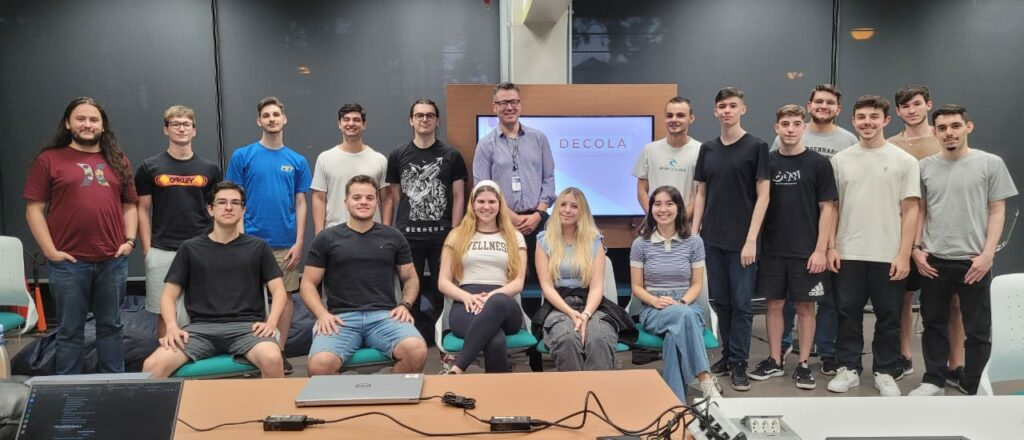
\includegraphics[width=1\linewidth]{conteudo//2 - ages I//conteudo//figures/decola-time.jpg}
    Fonte: Wiki do Projeto
    \label{fig:projeto-time-decola}
\end{figure}